\toclesssection{SCP 009 - Red Ice}
\addcontentsline{toc}{section}{SCP 009 - Red Ice}
\textbf{Item \#:} SCP-009

\textbf{Object Class:} Euclid

\begin{figure}[h]
\begin{center}
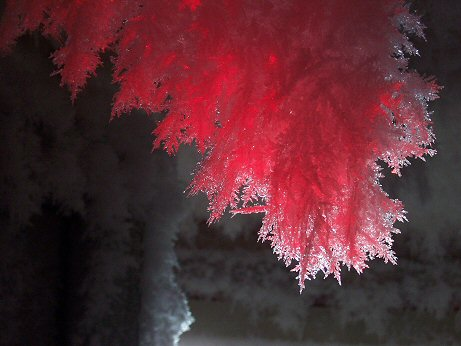
\includegraphics[scale=1.3]{scp/009.jpg}
\linebreak SCP-009 prior to recovery
\end{center}
\end{figure}


\textbf{Special Containment Procedures:} Subject is to be contained within a sealed storage tank of heat-resistant alloy with dimensions not less than 14m$^3$.

Under no circumstances should SCP-009 be exposed to temperatures in excess of 0°C when not undergoing testing, and no mundane liquids in a solid state (especially frozen water) shall be allowed within 30 meters of the subject's containment area. Subject's chamber is to be fitted with temperature sensors which shall be monitored at all times, and is to be kept refrigerated by no fewer than three (3) redundant cooling units. Any malfunction of sensors, or of coolant systems, is to be reported and repaired immediately.

If at any time the temperature in the containment area climbs above -5°C, the chamber is to be locked down immediately, and flooded with coolant until the temperature has been brought back down to between -30\degree C and -25\degree C. Atmosphere must be evacuated from the containment area when personnel are present within, and any water vapor present must be filtered and kept in the same conditions as detailed herein for no fewer than 24 hours. Any vapor displaying properties of SCP-009 is to be quarantined and added to the containment area as soon as possible.
\newpage
All personnel interacting with or observing the subject must wear full environmental protection suits. All personnel leaving the containment chamber must undergo dehydration of all gear, research materials, and other objects contacting SCP-009's chamber. If contamination is discovered, no material or personnel shall be permitted to exit, and a Level 2 lock-down of the containment area shall commence. Lethal force is authorized in cases of dire need, but all security forces are strongly advised to remain as far away from their targets as possible, to minimize the chance of contact with fluids contaminated by SCP-009.

\textbf{Description:} SCP-009 is approximately 3,700 liters of a substance which exhibits a number of unique properties. While small amounts of the substance, in all phases, are as colorless as mundane water, en masse it takes on a distinct deep red hue.

Its most notable property, however, is the fact that SCP-009's reaction to temperature extremes is exactly opposite that of standard H$_{2}$O: the subject assumes a liquid phase at temperatures between -100\degree C and 0\degree C, and converts into a solid state above those temperatures. At temperatures below -100\degree C, SCP-009 vaporizes into a gaseous phase similar to steam, though it still retains its red coloration when put under high pressure.

Examinations of the atomic structure of SCP-009 have proved inconclusive. Tests indicate that the subject is composed of the same combination of hydrogen and oxygen as normal water, leaving researchers to speculate that the source of the subject's abnormalities may be the atoms themselves. Dr. \censor{XXXXXX} has suggested that the subject may have originated in or been altered by another reality in which the laws of physics are inverted.

This theory may have some merit in light of SCP-009's marked ability to "assimilate" natural water into its mass. If placed in physical contact with any aqueous solution (be it ice, salt water, or water vapor in air), SCP-009 will "spread" and contaminate any H2O in said solution, causing it to exhibit the subject's properties. Though this capacity is present in all phases, it has been observed to progress most slowly (and thus be most containable) in the liquid phase.

If the subject comes in contact with any biological source of heat, it begins a runaway reaction in which the living organism's bodily fluids are rapidly converted to SCP-009 and promptly frozen by their own body heat (because of their generally high core temperatures, mammals are particularly susceptible). Because SCP-009 produces heat while freezing (at the same rate mundane ice consumes heat while melting), the process is self-perpetuating until all available moisture is converted, or until it is halted by external interference.
\newpage
Experiments on D-Class personnel have illustrated the process of conversion by the subject, which has been condensed down to a series of steps:

1. Initial Exposure: Subject is exposed to SCP-009, and it begins converting any water present on the exposed surface (usually skin) to exhibit its properties. Presence of mist, fog, snow, or other solid or vaporous water greatly accelerates this process.

2. Surface Conversion: A thin layer of frost forms on the exposed area as body heat and heat produced by SCP-009 raise its temperature above freezing. Progression to this step can take anywhere from five (5) minutes to one (1) hour, depending on victim's body temperature. At this stage, freezing has begun progressing through the initial layers of the epidermis and soon reaches live cells.

3. Deep Tissue Conversion: Exponential increase in temperature of SCP-009 causes expansion of ice crystals throughout the victim's body, resulting in widespread perforation of internal cell structure. Actual blood loss is minimal at this stage due to the crystals filling the puncture wounds, allowing subjects to remain alive and conscious for up to \censor{XX} hours.

4. \expunged

5. Death: Multiple organ failure and exsanguination via systemic crystallization.

Testing on D-Class personnel was discontinued as of\linebreak 4/23/20\censor{XX}.

\textbf{Addendum: Circumstances of Retrieval:} Subject was found in \censor{XXXX}, Alaska, on 11/05/19\censor{XX}. The Foundation got involved after reports were obtained from the native \censor{XXXX} Tribe, who came across the mangled bodies of a team of seal hunters which had apparently been ship-wrecked \censor{XX} kilometers from the village.

All victims were found encased in red ice. Cause of death recorded as internal bleeding. On victims whose features were sufficiently intact, expressions of panic and intense pain were observed. It is surmised that the low ambient temperatures in the area retarded the freezing process. This prolonged the time to total conversion by \censor{XX} hours, and allowed the victims to remain conscious until \expunged.

\textbf{Addendum:} 12/16/20\censor{XX}

Super-cooling of SCP-009 for the purposes of experimentation is disallowed until further notice. Personnel are advised that liquid nitrogen is only to be used on the subject in controlled amounts, and only until temperatures have reached acceptable levels.

Related note: Possible application of SCP-009 in cold fusion research pending evaluation.